\section{Maria Psarakis}
\begin{figure}
    \centering
    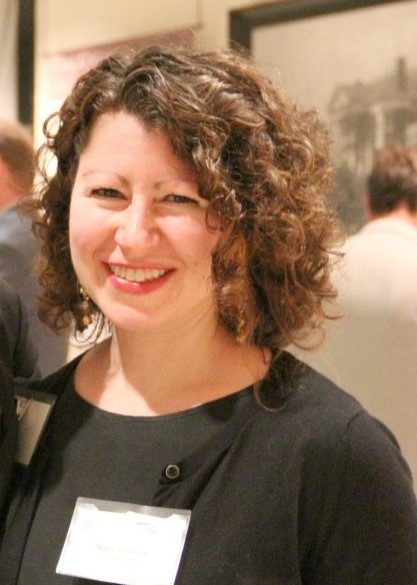
\includegraphics[scale=0.5]{mpsaraki.jpg}
    %\caption{}
    %\label{fig:my_label}
\end{figure}

I am in the master's program studying cybersecurity. I am currently in the process of a career transition; my previous job was as a Russian and French linguist. I am planning on graduating in May 2021, with the main goal of combining the skills I am getting now in this program in cybersecurity with the foreign languages I know.

In terms of research, I spent the summer doing the first three credits of my master's thesis, and I am looking to complete and defend it during this Fall semester. I am investigating the vulnerabilities of internet voting, comparing different implementations, and testing the code in one open-source implementation to see if it is in fact secure in terms of the security properties it claims to ensure.

To tell you a bit more about my background, I've lived in many different countries, mainly in Western Europe. I've had the opportunity to travel to Africa and Central Asia. I was also a "human test subject" at NASA, and tested exercise equipment that is now on the International Space Station.

Outside of my career pursuits, I am passionate about animal rescue, and have been a volunteer at the Humane Society for nearly five years.

\textbf{Question (from Cassandra Putman):} You went from learning different human languages to learning different programming languages.  Which one do you find more challenging to learn?
\textbf{Answer to Cassandra Putman from Maria Psarakis:} Thanks for your question! I think I would have to say programming languages, mainly because I haven't had as much practice. That may be the key to both, is just lots of practice.